\section{消息依赖密钥安全}
%可以先介绍Wee的~\cite{Wee-PKC-2016}, 再介绍韩帅等的~\cite{HLL-ASIACRYPT-2016}. 

在公钥加密方案的安全模型中, 加密的消息一般是根据明文空间的某一概率分布选择的, 而与加密算法的私钥无关.然而在硬盘加密、匿名证书系统等应用环境下, 加密的消息与私钥有关甚至是私钥本身(如$f(sk)$, 其中$f$是一个从密钥空间到消息空间的函数.), 传统的安全模型并不能完全满足这类应用的需求. 实际上, 早在1984年Goldwasser和Micali~\cite{GM-JCSS-1984}提出概率加密方案时, 已经指出当加密的消息与密钥相关时, 无法保证方案的语义安全性. Black等人~\cite{BRS2002}将加密这种特别消息下的安全性称之为消息依赖密钥安全性(Key-Dependent Message Security, 简称KDM安全性)或者是Camenisch和Lysyanskaya~\cite{CL-EUROCRYPT-2001}针对多用户环境下的循环加密安全性(Circular Security). KDM安全性不仅能够解决实际应用中面临的安全问题, 而且还可以用于设计CCA安全的公钥加密方案和单向陷门函数~\cite{KMT-JOC-2022}.

在KDM安全性中, 不同的应用环境要求被加密的私钥函数$f$有所不同. 一般情况下, 简单的仿射函数即可满足需求. 然而, 即使在这种情况下, 设计KDM安全的公钥加密方案也是相当困难的. 2008年,Boneh等人~\cite{BHHO2008}利用私钥的密文公开可计算性的思想, 提出了第一个标准模型下基于DDH困难问题的循环加密方案. 后来, 学者们基于类似思想提出了不同计算假设下的KDM安全的加密方案~\cite{ACPS2009,BG2010,MTY2011-EUROCRYPT}. 2016年, Wee将这些方案的设计思想统一为同态平滑投影哈希技术~\cite{Wee-PKC-2016}. 尽管这些方案具有KDM安全性, 但是仅能抵抗选择明文攻击. 对于选择密文攻击, 由于私钥的密文公开可计算性与解密服务之间是相矛盾的, 因此设计抗选择密文攻击的KMD安全加密方案更具有挑战性. 一种似乎万能效率不太高的方式就是利用从CPA到CCA转化的``Naor-Yung双加密''模式~\cite{CCS2009}. 另一种方式就寻找特殊的密码工具实现KDM-CCA安全性, 如有损代数过滤器(Lossy Algebraic Filter)~\cite{Hofheinz2013-EUROCRYPT}、辅助输入安全的认证加密(Authenticated Encryption with Auxiliary-Input, 简称AIAE)~\cite{HLL-ASIACRYPT-2016}等. 

本节内容主要介绍消息依赖密钥安全性的模型, 基于同态平滑投影哈希技术的KDM-CPA安全设计方法, 基于辅助输入安全认证加密技术的KDM-CCA安全设计方法, 以及具有KDM-CCA安全的Cramer-Shoup加密方案.

\subsection{安全模型}
消息依赖密钥加密可以看作是一种特殊的密钥泄漏函数. 在消息依赖密钥安全模型中, 存在一个与密钥相关的函数集合$\mathcal{F}$将(一组)密钥映射到消息空间. 与密钥泄漏安全模型不同, 消息依赖密钥加密泄漏的不是该密钥的函数值而是它的密文, 比如$\mathsf{Encrypt}(pk,f(sk))$.

在给出消息依赖密钥安全模型的形式化定义之前, 先介绍一个简单的反例说明并不是所有语义安全的加密方案都是KDM安全的~\cite{CGH2012}. 假设$\text{PKE} = (\mathsf{Setup}, \mathsf{KeyGen}, \mathsf{Encrypt}, \mathsf{Decrypt})$是任意一个语义安全的加密方案. 在该方案的基础上构造一个新的加密方案$\text{PKE}' = (\mathsf{Setup}', \mathsf{KeyGen}', \mathsf{Encrypt}', \mathsf{Decrypt}')$, 其中$\mathsf{Setup}'$和$\mathsf{KeyGen}'$与原方案一样, $\mathsf{Encrypt}'$和$\mathsf{Decrypt}'$的定义如下:
\begin{align*}
\mathsf{Encrypt}'(M)&=\left\{\begin{array}{ll}
\mathsf{Encrypt}(M)||0 & \textrm{if $M\neq sk$}\\
\mathsf{Encrypt}(M)||1 & \textrm{if $M=sk$}
\end{array}\right. &
\mathsf{Decrypt}'(C||b)&=\left\{\begin{array}{ll}
\mathsf{Decrypt}(C) & \textrm{if $b=0$}\\
sk & \textrm{if $b=1$}
\end{array}\right..
\end{align*}
显然, 在语义安全性模型中, 消息是从明文空间中公开选取的, 等于私钥$sk$的概率是可忽略的, 密文的形式永远是$\mathsf{Encrypt}(M)||0$, 所以$\text{PKE}'$仍然是语义安全的. 但是在消息依赖密钥加密模型中, 消息等于或不等于$sk$时的密文形式是可以直接区分的, 所以$\text{PKE}'$不具有消息依赖密钥安全性。

\begin{definition} [KDM-CCA安全性]
对于任意$n \in \mathbb{N}$, 令$\mathcal{F} = \{f: \mathcal{SK}^n \rightarrow \mathcal{M}\}$是一个从$n$维密钥空间到消息空间的KDM函数族. 定义公钥加密方案$\text{PKE}$的KDM-CCA敌手$\mathcal{A}$的优势函数如下: 
\begin{displaymath}
	\mathsf{Adv}_{\mathcal{A}, \mathcal{F}, \text{PKE}}^{\text{KDM-CCA}}(\kappa) = \left| \Pr \left[ \beta' = \beta:~
	\begin{array}{ll}
		& pp \leftarrow \mathsf{Setup}(1^\kappa); \\		
		& (pk_i, sk_i) \leftarrow \mathsf{KeyGen}(pp), \forall i \in [n];\\
		& \text{Set } \mathsf{CL} = \empty, \overrightarrow{pk} = (pk_1, \ldots, pk_n), \overrightarrow{sk} = (sk_1, \ldots, sk_n); \\
		& \beta \sample \{0,1\};\\ 
		& \beta' \leftarrow \mathcal{A}^{\blue{\mathcal{O}_{\text{Enc}}}(\cdot), \blue{\mathcal{O}_{\text{Dec}}}(\cdot)}(pp, \overrightarrow{pk});
	\end{array} 
\right] - \frac{1}{2} \right|,
\end{displaymath}
其中, 加密谕言机和解密谕言机的定义如下:
\begin{itemize}
\item 加密谕言机$\mathcal{O}_{\text{Enc}}(\cdot)$: 输入$(i, f)$, 其中$i \in [n]$, $f \in \mathcal{F}$, 如果$\beta = 0$, 返回$C=\mathsf{Encrypt}(pk_i, f(\overrightarrow{sk}))$; 如果$\beta = 1$, 返回$C=\mathsf{Encrypt}(pk_i, 0^{|\mathcal{M}|})$. 最后, 将$(i, C)$添加至密文列表$\mathsf{CL}$中.

\item 解密谕言机$\mathcal{O}_{\text{Dnc}}(\cdot)$: 输入$(i, C)$, 其中$i \in [n]$. 如果$(i, C) \in \mathsf{CL}$, 返回$\bot$; 否则, 返回$\mathsf{Dncrypt}(sk_i, C)$.
\end{itemize}

上述定义中, 如果对于任意的PPT敌手$\mathcal{A}$, 优势函数$\mathsf{Adv}_{\mathcal{A}, \Phi, \text{PKE}}^{\text{KDM-CCA}}(\kappa)$是可忽略的, 则称公钥加密方案$\text{PKE}$是$\mathcal{F}$-KDM-CCA安全的.
\end{definition}

\begin{note}
KDM-CCA安全模型说明了敌手在解密服务的帮助下, 也无法区分一组密文是加密的私钥相关函数值还是某一固定消息, 例如$0^{|\mathcal{M}|}$. 若不允许敌手进行解密询问, 则上述模型即是KDM或KDM-CPA全性的定义. 不同类型的函数族$\mathcal{F}$对于是实现KDM安全性的难度是不同的. 若$\mathcal{F}$是常数函数族$\{f_M: \overrightarrow{sk} \rightarrow M\}_{M\in\mathcal{M}}$, 则KDM-CPA安全性等价于传统的语义安全性(IND-CPA). 而KDM-CCA安全性即是传统的IND-CCA安全性. 若$\mathcal{F}$是选择函数族$\{f_i:\overrightarrow{sk} \rightarrow sk_i \}$,此时的KDM安全性也称之为循环加密安全性(Circular Security).
\end{note}

\subsection{Wee16方案}
\subsubsection{同态平滑仿射哈希}
平滑仿射哈希(Smooth Projective Hashing, 简称SPH)是Cramer和Shoup在2002年提出的一种哈希证明系统~\cite{CS-EUROCRYPT-2002}. 令$\text{HPS} = (\mathsf{Setup}, \mathsf{KeyGen}, \mathsf{PrivEval}, \mathsf{PubEval})$是一个哈希证明系统. 运行$\mathsf{Setup}(1^\kappa)$输出一组公开参数$pp = (\mathsf{H}, SK, PK, X, L, W, \Pi, \alpha)$, 其中$X$定义了一个元素集合, $L \subset X$表示合法元素集合, $X \setminus L$表示非法元素集合, 合法元素与非法元素在计算上是不可区分的. 运行$\mathsf{KeyGen}(pp)$将输出一对密钥$(pk, sk)$, 其中$sk \sample SK$, $pk = \alpha (sk)$也成为仿射密钥.

\begin{trivlist}
\item \textbf{同态平滑仿射哈希:} 是一组定义在$\{\mathsf{H}_{sk}: X \rightarrow \Pi\}$上的平滑仿射哈希. 类似平滑仿射哈希, 除了具有私有可计算、公开可计算、平滑性等性质外, 还需要具有同态性. 具体如下:
\begin{itemize}
\item 私有可计算性(Private Evaluation): 对于任意$x \in X$, 存在算法$\mathsf{PrivEval}(sk, x)$, 输出$\pi = \mathsf{H}_{sk}(x)$.

\item 公开可计算性(Public Evaluation): 对于任意$x \in L$以及相应的$w$, 存在算法$\mathsf{PubEval}(pk, x, w)$, 输出$\pi = \mathsf{H}_{sk}(x)$.

\item 平滑性(Smoothness): $\mathsf{H}_{sk}(\cdot)$在输入$x \sample X$时的输出与$\Pi$上的均匀分布统计接近, 即: 
\begin{equation*}
    (pk, \mathsf{H}_{sk}(x)) \approx_s (pk, \pi)
\end{equation*}
其中$(pk, sk) \leftarrow \mathsf{KeyGen}(pp)$, $\pi \sample \Pi$.

\item 同态性(Homomorphism): 对于所有$sk \in SK$和所有$x_0, x_1 \in X$, 我们有$\mathsf{H}_{sk}(x_0)\cdot \mathsf{H}_{sk}(x_1) = \mathsf{H}_{sk}(x_0 \cdot x_1)$.   
\end{itemize}
\end{trivlist}

\subsubsection{基于同态平滑仿射哈希的KDM-CPA方案}
\begin{construction}[基于HSPH的KDM-CPA方案]\label{construction:Wee16-KDM}
除了使用工具同态平滑投影哈希外, 我们还需要一个从消息空间$\mathcal{M}$到哈希值空间$\Pi$的一个公开可计算且可逆的映射$\phi: \mathcal{M} \rightarrow \Pi$.
\begin{itemize}
\item $\mathsf{Setup}(1^\kappa)$: 运行$pp \leftarrow \text{HPS}.\mathsf{Setup}(1^\kappa)$, 输出系统参数$pp = (\mathsf{H}, SK, PK, X, L, W, \Pi, \alpha)$.

\item $\mathsf{KeyGen}(pp)$: 运行$(pk, sk) \leftarrow \text{HPS}.\mathsf{KeyGen}(pp)$, 输出公钥$pk$和私钥$sk$, 其中$sk \sample SK$, $pk = \alpha (sk)$. 
  
\item $\mathsf{Encrypt}(pk, M)$: 以公钥$pk$和明文$M \in \mathcal{M}$为输入, 执行如下步骤:
\begin{enumerate}
    \item 运行$(x, w) \leftarrow \mathsf{SampR}(r)$生成随机实例$x \in L$及相应的证据$w$, 其中$r$为采用时使用的随机数; 
    \item 通过$\text{HPS}.\mathsf{PubEval}(pk, x, w)$计算实例$x$的哈希证明$\pi = \mathsf{H}_{sk}(x)$;
    \item 计算$\psi = \pi \cdot \phi(M)$;
    \item 输出密文$C = (x, \psi)$. 
\end{enumerate} 

\item $\mathsf{Decrypt}(sk, C)$: 以私钥$sk$和密文$C = (x, \psi)$为输入, 计算$M' = \phi^{-1}(\mathsf{H}_{sk}(x)^{-1}\cdot \psi)$并返回明文$M'$. 
\end{itemize}
\end{construction}

\begin{trivlist}
\item \textbf{正确性.} 方案的正确性可由仿射哈希的完备性保证. 安全性由如下定理保证.
\end{trivlist}
\begin{theorem}\label{theorem:Wee-KDM}
假设$\mathsf{H}_{sk}(\cdot)$是一个定义在$X$上的仿射哈希函数, 满足平滑性和同态性, 并且$L \subseteq X$上的SMP困难问题成立, 那么构造~\ref{construction:Wee16-KDM}中的PKE方案是$\mathcal{F}$-KDM-CPA安全的, 其中$\mathcal{F} = \{f_{e, k}: sk \rightarrow \phi^{-1}(\mathsf{H}_{sk}(e)\cdot k)~|~e \in X, k \in \Pi\}$.
\end{theorem}

定理~\ref{theorem:Wee-KDM}的证明思路主要是将密钥函数值$f_{x, \pi}(sk)$的密文转化为函数参数$(x, \pi)$的密文, 由此使得KDM密文与私钥$sk$无关. 转化的技术是仿射哈希的同态性. 即, 将$f_{x, \pi}(sk)$的密文:
\[
\mathsf{Encrypt}(pk, f_{e, k}(sk)) = (x,\mathsf{H}_{sk}(x) \cdot f_{e, k}(sk))
\]
转化为
\begin{equation}\label{eq:kem-CT}
\mathsf{Encrypt}(pk, f_{e, k}(sk)) = (x \cdot e^{-1},\text{HPS}.\mathsf{PubEval}(pk, x, w) \cdot k).
\end{equation}
从而使得挑战者在不知道私钥$sk$的情况下, 也可以回答敌手的KDM加密询问. 下面给出详细的证明过程.
\begin{proof}
令$S_i$表示敌手在$\text{Game}_i$中的成功事件. 以游戏序列的方式组织证明如下: 
\begin{trivlist}
\item $\text{Game}_0$: 该游戏是标准的KDM-CPA游戏, 挑战者$\mathcal{CH}$和敌手$\mathcal{A}$交互如下: 
\begin{itemize}
\item 初始化: $\mathcal{CH}$运行$\mathsf{Setup}(1^\kappa)$生成公开参数$pp$, 
		同时运行$\mathsf{KeyGen}(pp)$生成公私钥对$(pk, sk)$. $\mathcal{CH}$将$(pp, pk)$发送给$\mathcal{A}$. 

\item 挑战: $\mathcal{CH}$选择随机比特$\beta \in \{0,1\}$.

\item 询问: 对于敌手的任意询问$f_{e, k} \in \mathcal{F}$, $\mathcal{CH}$作如下计算: 
\begin{enumerate}
    \item 如果$\beta = 0$, $\mathcal{CH}$随机选择$x \in L$及相应的证据$w$, 计算密文$C = (x, \psi)$, 其中
\[
\psi = \text{HPS}.\mathsf{PubEval}(pk, x, w) \cdot \phi(f_{e, k}(sk)) = \text{HPS}.\mathsf{PubEval}(pk, x, w) \cdot \mathsf{H}_{sk}(e)\cdot k.
\]
    \item 如果$\beta = 1$, $\mathcal{CH}$随机选择$x \in L$及相应的证据$w$, 计算密文$C = (x, \psi)$, 其中
\[
\psi = \text{HPS}.\mathsf{PubEval}(pk, x, w) \cdot \phi(0^{|\mathcal{M}|}).
\]
    \item 最后, $\mathcal{CH}$将密文$C = (x, \psi)$返回给敌手. 
\end{enumerate} 

\item 猜测: $\mathcal{A}$输出对$\beta$的猜测$\beta'$. $\mathcal{A}$成功当且仅当$\beta' = \beta$. 
\end{itemize} 
根据定义, 我们有: 
\begin{equation*}
	\mathsf{Adv}_{\mathcal{A}, \mathcal{F}, \text{PKE}}^{\text{KDM-CPA}}(\kappa) = |\Pr[S_0] - 1/2|
\end{equation*}

\item $\text{Game}_1$: 该游戏与$\text{Game}_0$的唯一不同在于$\beta = 0$时加密谕言机的工作方式. 具体地, 对于敌手的任意加密询问$f \in \mathcal{F}$, 当$\beta = 0$时, $\mathcal{CH}$返回形如公式~\ref{eq:kem-CT}中的密文. 

假设$\mathcal{A}$询问加密谕言机的次数最多为$Q$次, 我们可以利用混合游戏的思想在$\text{Game}_0$和$\text{Game}_1$之间定义$Q-1$个混合游戏$\text{Game}_{0,i}$,其中$i \in \{1, \ldots, Q-1\}$. 在$\text{Game}_{0,i}$中, 当$\beta = 0$时, $\mathcal{A}$的前$i$个询问的密文是公式~\ref{eq:kem-CT}中的形式, 而后$Q-i$次询问的密文按正常方式加密得来. 显然, $\text{Game}_{0,0} = \text{Game}_0$, $\text{Game}_{0,Q} = \text{Game}_1$. 对于任意的$i$, 敌手在两个连续游戏中的视图是不可区分的, 即$
\text{Game}_{0, i-1} \approx \text{Game}_{0, i}$. 这是因为
\begin{displaymath}
\begin{array}{lll}
  & \mathsf{Encrypt}(pk, f_{e, k}(sk)) & \\
= & (x, \text{HPS}.\mathsf{PubEval}(pk, x, w) \cdot \mathsf{H}_{sk}(e) \cdot k) & :  (x, w)\leftarrow \mathsf{SampR}(r)\\
= & (x, \mathsf{H}_{sk}(x) \cdot \mathsf{H}_{sk}(e) \cdot k) & :  \text{仿射性质} \\
\approx_c & (x, \mathsf{H}_{sk}(x) \cdot \mathsf{H}_{sk}(e) \cdot k) & :  x\sample X, \text{SMP问题} \\
= & (x, \mathsf{H}_{sk}(x \cdot e) \cdot k) & :  x\sample X, \text{同态性质} \\
= & (x \cdot e^{-1}, \mathsf{H}_{sk}(x) \cdot k) & :  x\sample X\\
\approx_c & (x \cdot e^{-1}, \mathsf{H}_{sk}(x) \cdot k) & :  (x, w)\leftarrow \mathsf{SampR}(r)\\
= & (x \cdot e^{-1}, \text{HPS}.\mathsf{PubEval}(pk, x, w) \cdot k) & :  (x, w)\leftarrow \mathsf{SampR}(r), \text{仿射性质}\\
\end{array}
\end{displaymath}
特别注意, 在上式的演进过程中, 密钥$s$是完全公开的. 因此, 在前$i$次询问时, $\mathcal{CH}$可以用公钥和KDM函数$f_{e, k}$计算密文$(x \cdot e^{-1}, \text{HPS}.\mathsf{PubEval}(pk, x, w) \cdot k)$, 而对于后$Q-i$次询问, $\mathcal{CH}$可以用私钥$sk$和KDM函数$f_{e, k}$计算密文$\mathsf{Encrypt}(pk, f_{e, k}(sk))$. 

由此可知, 
\[
|\Pr[S_1] - \Pr[S_2]| \leq \mathsf{negl}(\kappa).
\]

\item $\text{Game}_2$: 该游戏与$\text{Game}_1$的唯一不同在于$\beta = 0$时加密谕言机的工作方式. 具体地, 对于敌手的任意加密询问$f \in \mathcal{F}$, 当$\beta = 0$时, $\mathcal{CH}$返回一个随机密文$(x, \psi)$, 其中$x \sample X$, $\psi \sample \Pi$. 在$\text{Game}_1$中, 由于KDM密文可以由公钥$pk$和KDM函数的参数$(e, k)$公开计算, 因此我们只需要证明
\[
(x \cdot e^{-1}, \text{HPS}.\mathsf{PubEval}(pk, x, w) \cdot k) \approx (x, \psi)
\]
其中$(x, w)\leftarrow \mathsf{SampR}(r)$, $x \sample X$, $\psi \sample \Pi$. 这是因为
\begin{displaymath}
\begin{array}{lll}
  & (x \cdot e^{-1}, \text{HPS}.\mathsf{PubEval}(pk, x, w) \cdot k) & :  (x, w)\leftarrow \mathsf{SampR}(r) \\
\approx_c & (x \cdot e^{-1}, \mathsf{H}_{sk}(x) \cdot k) & :  (x, w)\leftarrow \mathsf{SampR}(r), \text{仿射性质}\\
\approx_c & (x \cdot e^{-1}, \mathsf{H}_{sk}(x) \cdot k) & :  x \sample X, \text{SMP性质}\\
\approx_s & (x \cdot e^{-1}, \pi \cdot k) & :  x \sample X, \pi \sample \Pi, \text{平滑性}\\
= & (x, \psi) & :  x \sample X, \psi \sample \Pi      \\
\end{array}
\end{displaymath}
由此可知, 在游戏$\text{Game}_2$中, 当$\beta = 0$, 加密谕言机返回的都是随机密文, 与KDM函数值$f_{e, k}(sk)$无关.

\item $\text{Game}_3$: 该游戏与$\text{Game}_2$的唯一不同在于$\beta = 1$时加密谕言机的工作方式. 具体地, 对于敌手的任意加密询问$f \in \mathcal{F}$, 当$\beta = 1$时, $\mathcal{CH}$返回一个随机密文$(x, \psi)$, 其中$x \sample X$, $\psi \sample \Pi$. 我们知道, 当$\beta = 1$时, 加密谕言机返回的密文形式是$\mathsf{Encrypt}(pk, 0^{|\mathcal{M}|})$. 利用仿射哈希的平滑性, 可以直接证明消息$0^{|\mathcal{M}|}$的密文与一个随机密文是不可区分的, 即
\[
|\Pr[S_2] - \Pr[S_3]| \leq \mathsf{negl}(\kappa).
\]

在$\text{Game}_3$中, 不管$\beta = 0$还是$\beta = 1$, 加密谕言机返回的都是一个随机密文, 与挑战比特$\beta$完全无关. 由此, 我们可得
\[
\Pr[S_3] = 1/2.
\]
\end{trivlist}

综上, 定理得证! \qed
\end{proof}

\subsection{HLL16方案}
2015年, Lu、Li和Jia~\cite{LLJ2015}构造了第一个高效的、密文紧凑的KDM$[\Faff]$-CCA安全公钥加密方案, 其密文甚至只包括7个群元素. 该方案的安全性同时基于DDH和DCR这两个假设, 所支持的私钥函数集合为仿射函数集合$\Faff$. 该方案使用了一个很重要的工具, 即\emph{RKA安全的认证加密方案$\overline{\mathsf{AE}}$}. 用在RKA攻击下同时具有不可区分性(IND-${\F}$-RKA)和完整性(INT-$\mathcal{F}$-RKA)的认证加密方案, 构造出了KDM-CCA安全的公钥加密方案. LLJ方案的KDM$[\mathcal{F}_{\text{aff}}]$-CCA安全性十分依赖于组件$\overline{\mathsf{AE}}$的INT-$\Faff$-RKA安全性(参见文献~\cite{LLJ2015}定义2). 然而LLJ方案中使用的认证加密方案在安全性上存在一定的缺陷, 从而导致LLJ方案的KDM$[\Faff]$-CCA安全性证明的失败.

2016年, Han、Liu和Lyu~\cite{HLL-ASIACRYPT-2016}针对仿射函数集合和多项式函数集合, 分别构造高效的、密文紧凑的KDM$[{\Faff}]$-CCA安全公钥加密方案以及高效的KDM$[\Fpolyd]$-CCA安全公钥加密方案. 该方案提出一个全新的密码原语,即支持辅助输入的认证加密方案$\AIAE$, 并为其定义了弱RKA安全性. 该新原语成为了实现KDM-CCA安全公钥加密方案的必要工具.

下面主要介绍AIAE的概念、基于AIAE的KDM-CCA安全公钥加密方案的通用设计方法、支持仿射函数集的KDM-CCA安全公钥加密方案和支持多项式函数集的KDM-CCA安全公钥加密方案.

\subsubsection{支持辅助输入的认证加密方案}
下面介绍支持辅助输入的认证加密方案$\AIAE$的形式化定义及其弱RKA安全性. 基于传统的认证加密方案和具有密钥同态性质的带标签哈希证明系统, 给出$\AIAE$的通用构造, 并基于DDH假设给出$\AIAE$的具体实例.

\begin{definition}[支持辅助输入的认证加密方案]\label{defn:AIAE}
一个支持辅助输入的认证加密方案$\text{AIAE} = (\mathsf{Setup}, \mathsf{Encrypt}, \mathsf{Decrypt})$由三个PPT算法组成:
\begin{itemize}
\item $\mathsf{Setup}(1^\kappa)$: 输入安全参数$\kappa$, 输出一个公开参数$pp_{\text{AIAE}}$. 公开参数$pp_{\text{AIAE}}$隐含地定义了一个密钥空间$\mathcal{K}_{\text{AIAE}}$、一个消息空间$\mathcal{M}$和一个辅助输入空间$\mathcal{AUX}$. 为了方便起见, 公开参数$pp_{\text{AIAE}}$会默认作为所有算法的一个输入.
\item $\mathsf{Encrypt}(k, m, aux)$: 以密钥$k \in \mathcal{K}_{\text{AIAE}}$、消息$m \in \mathcal{M}$和辅助输入$aux \in \mathcal{AUX}$为输入, 输出一个密文$C$.
\item $\mathsf{Decrypt}(k, C, aux)$: 以密钥$k \in \mathcal{K}_{\text{AIAE}}$、密文$C$和辅助输入$aux \in \mathcal{AUX}$为输入,输出一个消息$m \in \mathcal{M}$或者一个代表解密失败的符号$\bot$.
\end{itemize}
\end{definition}

\begin{trivlist}
\item \textbf{正确性.} 对所有$pp_{\text{AIAE}}\leftarrow \mathsf{Setup}(1^{\kappa})$、所有密钥$k \in \mathcal{K}_{\text{AIAE}}$、所有消息$m \in \mathcal{M}$和所有辅助输入$aux \in \mathcal{AUX}$, 满足$\mathsf{Decrypt}(k, \mathsf{EEncrypt}(k, m, aux), aux) = m$。
\end{trivlist}

\begin{note}
认证加密方案是一种私钥加密方案. 辅助输入的认证加密方案可以看作是一种辅助输入的私钥加密方案, 也可以看成是传统认证加密方案的一个扩展. 因为对于所有的系统参数$pp_{\text{AIAE}}$, 如果辅助输入空间$\mathcal{AUX}$都为空集, 则上述定义就退化为传统的认证加密方案.  
\end{note}


令$\F$为一族从$\mathcal{K}_{\text{AIAE}}$到$\mathcal{K}_{\text{AIAE}}$的函数. 我们通过图\ref{fig:AIAE-RKA}中的实验来定义AIAE的弱RKA安全性. 在$\mathsf{weak}$-$\mathsf{INT}$-$\F$-$\mathsf{RKA}$实验的\textsc{Finalize}程序中, 有一个用灰色背景标注的特殊规则.


\begin{definition}[AIAE的弱$\F$-RKA安全性]~\label{def:weak-RKA-AIAE}
一个支持辅助输入的认证加密方案AIAE是弱$\F$-RKA安全的, 如果它是IND-$\F$-RKA安全和弱INT-$\F$-RKA安全的, 即对于任意PPT敌手$\mathcal{A}$,满足条件
$$\mathsf{Adv}_{\text{AIAE}, \F, \mathcal{A}}^{\text{ind-rka}}(\kappa) := \big| \Pr[ \text{$\mathsf{IND}$-$\F$-$\mathsf{RKA}$}^{\mathcal{A}} \Rightarrow 1] - 1/2 \big| \leq \mathsf{negl}(\kappa),$$
$$\mathsf{Adv}_{\text{AIAE}, \F, \mathcal{A}}^{\text{weak-int-rka}}(\kappa) := \Pr[\text{$\mathsf{weak}$-$\mathsf{INT}$-$\F$-$\mathsf{RKA}$}^{\mathcal{A}} \Rightarrow 1] \leq \mathsf{negl}(\kappa),~$$
其中$\mathsf{IND}$-$\F$-$\mathsf{RKA}$和$\mathsf{weak}$-$\mathsf{INT}$-$\F$-$\mathsf{RKA}$是图\ref{fig:AIAE-RKA}中描述的实验.
\end{definition}

{\renewcommand{\baselinestretch}{1.2} \normalsize
\begin{figure}[hpt]
\centering
\scalebox{0.95}
{\begin{tabular}{|l || l|}
\hline
~\makecell[l]{
\underline{\textbf{程序} \textsc{Initialize}:} \\
$\prmAIAE \leftarrow \text{AIAE}.\mathsf{Setup}(1^{\kappa})$. ~\\
$k \sample {\KAIAE}$. \\
$\beta \sample \{0, 1\}$.  \hfill{// 挑战比特} \\
Return~ $\prmAIAE$. \\
~~\\
\underline{\textbf{程序} $\textsc{Enc}(f \in \F, m_0, m_1, aux)$:}  \\
如果$|m_0| \neq |m_1|$, Return~ $\bot$. \\
$\mathsf{aiae.ct} \leftarrow \text{AIAE}.\mathsf{Encrypt}(f(k), m_\beta, aux)$. \\
Return~ $\mathsf{aiae.ct}$.  \\
~~\\
\underline{\textbf{程序} $\textsc{Finalize}(\beta')$:} \\
Return~ $(\beta' = \beta)$. \\
}~ &
~\makecell[l]{
\underline{\textbf{程序} \textsc{Initialize}:} \\
$\prmAIAE \leftarrow \text{AIAE}.\mathsf{Setup}(1^{\kappa})$, ~$k \sample {\KAIAE}$. \\
Return~ $\prmAIAE$. \\
\vspace{-4pt} \\
\underline{\textbf{程序} $\textsc{Enc}(f \in \F, m, aux)$:}  \\
$\mathsf{aiae.ct} \leftarrow \text{AIAE}.\mathsf{Encrypt}(f(k), m, aux)$. \\
$\mathcal{Q}_{\text{ENC}} := \mathcal{Q}_{\text{ENC}} \cup \big\{ (f, \mathsf{aiae.ct}, aux) \big\}$. \\
{$\mathcal{Q}_{\text{AUXF}} := \mathcal{Q}_{\text{AUXF}} \cup \big\{ (f, aux) \big\}$.} \\
Return~ $\mathsf{aiae.ct}$.  \\
\vspace{-4pt} \\
\underline{\textbf{程序} $\textsc{Finalize}\big(f^* \in {\F}, \mathsf{aiae.ct}^*, aux^*\big)$:} \\ 
如果$\big(f^*, \mathsf{aiae.ct}^*, aux^*\big) \in \mathcal{Q}_{\text{ENC}}$, Return~ $0$. \\
\grabox{\makecell[l]{
如果存在$(f, aux) \in \mathcal{Q}_{\text{AUXF}}$使得  \\
~~~~$aux = aux^*$但$f \neq f^*$, Return~ $0$. \\
}} ~{// 特殊规则} \\
Return~ ($\text{AIAE}.\mathsf{Decrypt}(f^*(k), \mathsf{aiae.ct}^*, aux^*) \neq \bot$). \\
}~     \\\hline
\end{tabular}}
\caption{支持辅助输入认证加密方案$\AIAE$的$\mathsf{IND}$-$\F$-$\mathsf{RKA}$实验(左图)及$\mathsf{weak}$-$\mathsf{INT}$-$\F$-$\mathsf{RKA}$实验(右图)}\label{fig:AIAE-RKA}
\end{figure}}


\begin{note}
辅助输入的认证加密方案的弱RKA安全性实际上包含两个方面: 一是敌手在任意篡改密钥$f(k)$下两个长度相同消息的密文依然不可区分; 二是敌手在获得若干篡改密钥和若干消息的密文, 依然无法生成一个新消息或新辅助元素的合法密文.
\end{note}

\medskip\noindent\textbf{AIAE方案的通用构造:} 基于标准的认证加密方案和密钥同态的带标签哈希证明系统可以构造支持辅助输入认证加密方案AIAE. 使用的组件具体包括:
\begin{itemize}
\item 一个传统的(即不支持辅助输入的)认证加密方案, 记作$\text{AE} = (\mathsf{Setup}, \mathsf{Encrypt}, \mathsf{Decrypt})$, 其密钥空间为$\mathcal{K}$, 消息空间为$\mathcal{M}$;

\item 一个具有密钥同态性质的带标签哈希证明系统, 记作$\text{THPS} = (\mathsf{Setup}, \mathsf{KeyGen}, \mathsf{PrivEval}, \mathsf{PubEval})$, 其哈希值空间为$\mathcal{K}$、标签空间为$\mathcal{T}$, ;

\item 一个抗碰撞的哈希函数族, 记作$\mathcal{TCR} = \{\textsf{TCR}: \{0, 1\}^* \rightarrow \mathcal{T} \}$.
%$\mathcal{H} = \{ \textsf{H}: \{0, 1\}^* \rightarrow \calT \}$(参见定义\ref{defn:cr})。
\end{itemize}
在上述组件中, 要求THPS的哈希值空间与AE的密钥空间相匹配, 而THPS的标签空间与$\mathcal{H}$的值域相匹配.

Han等人设计的支持辅助输入认证加密方案$\text{AIAE} = (\mathsf{Setup}, \mathsf{Encrypt}, \mathsf{Decrypt})$见图\ref{fig:AIAE-Con}, 其密钥空间为$\mathcal{K}_{\text{AIAE}} := \mathcal{SK}$、消息空间为$\mathcal{M}$、辅助输入空间为$\mathcal{AUX} = \{0, 1\}^*$.

{\renewcommand{\baselinestretch}{1.2} \normalsize
\begin{figure}[ht]
\centering
{\begin{tabular}{|c|c|c|}
\hline
~\makecell[l]{
\underline{$\text{AIAE}.\mathsf{Setup}(1^\kappa)$:}  \\
$pp_{\text{THPS}} \leftarrow \text{THPS}.\mathsf{Setup}(1^{\kappa})$. \\
$pp_{\text{AE}} \leftarrow \text{AE}.\mathsf{Setup}(1^{\kappa})$. \\
$\mathsf{TCR} \leftarrow \mathcal{TCR}$.  \\
$pp_{\text{AIAE}} := (pp_{\text{THPS}}, pp_{\text{AE}}, \mathsf{TCR})$. \\
Return~ $pp_{\text{AIAE}}$. \\
}~     &
~\makecell[l]{
\underline{$\text{AIAE}.\mathsf{Encrypt}(sk, m, aux)$:} \\
$x \sample L$及证据$w$. \\
$t \leftarrow \textsf{TCR}(x, aux) \in \mathcal{T}$. \\
$k \leftarrow  \mathsf{H}_{sk}(x, t) \in \mathcal{K}$. \\
$\chi \leftarrow \text{AE}.\mathsf{Encrypt}(k, m)$. \\
Return~ $\langle x, \chi \rangle$. \\
}~     &
~\makecell[l]{
\underline{$\text{AIAE}.\mathsf{Decryp}(sk, \langle  x, \chi \rangle, aux)$:} \\
如果$x \notin X$, ~Return~ $\bot$. \\
$t := \textsf{TCR}(x, aux) \in \mathcal{T}$. \\
$k := \mathsf{H}_{sk}(x, t)   \in \mathcal{K}$. \\
$m / \bot \leftarrow \text{AE}.\mathsf{Decrypt}(k, \chi)$. \\
Return~ $m / \bot$. \\
}~        \\\hline
\end{tabular}}\caption{支持辅助输入认证加密方案AIAE的通用构造}\label{fig:AIAE-Con}
\end{figure}
}

根据AE的正确性, 可以直接验证AIAE的正确性. 方案的弱$\F_{\text{raff}}$-RKA安全性由定理~\ref{thm:AIAE-RKA}保证, 其中$\F_{\text{raff}}$是受限仿射函数集合, 定义为: $\F_{\text{raff}}: = \big\{f_{(a, b)}: \mathsf{sk} \longmapsto a \cdot \mathsf{sk}  + b \in \mathcal{SK} ~\big|~a \in \mathbb{Z}_{| \mathcal{K} |}^*, b, \mathcal{sk} \in \mathcal{SK} \big\}$.
\begin{theorem} \label{thm:AIAE-RKA}
如果(i)AE是OT安全的;
(ii)THPS是2-universal、密钥同态的且SMP问题困难;
(iii)TCR是抗碰撞的;
则图\ref{fig:AIAE-Con}中构造的AIAE方案是弱$\F_{\text{raff}}$-RKA安全的.
\end{theorem}

上述定理的证明请参考博士论文~\cite{Han2019}定理3.1的证明.

\medskip\noindent\textbf{AIAE的实例化方案.} 2015年, Qin、Liu和Chen~\cite{QLC-IET-IFS-2015}基于$d$-Linear假设构造了一个带标签哈希证明系统. 2019年, Han将该哈希证明系统进一步扩展为具有\emph{密钥同态}性质的带标签哈希证明系统THPS, 并基于DDH困难假设证明了THPS的相关性质, 如图~\ref{fig:THPS-Con}所示. 将该哈希证明系统带入到上述通用构造中, 即可以得到一个基于DDH问题的支持辅助输入认证加密方案.
{\renewcommand{\baselinestretch}{1.2} \normalsize
%\setlength\tabcolsep{4pt}
\begin{figure}[htp]
\centering
%\scalebox{0.95}
{\begin{tabular}{|l|l|}
\hline
\multicolumn{2}{|l|}
{\makecell[l]{
\vspace{-11pt} \\
\underline{$pp_{\text{THPS}}  \leftarrow {\text{THPS}}\mathsf{.Setup}(1^\kappa)$:}  \\
\vspace{-11pt} \\
$(N, p, q) \leftarrow \mathsf{GenN}(1^{\kappa})$,   \\
~~~~ 即选取两个{$\kappa$}比特的安全素数$p$和$q$使得$2pq + 1$也是素数且$N:=pq$. \\
$\bar{N} := 2N + 1$. ~~${g}_1, {g}_2 \leftarrow \mathbb{QR}_{\bar{N}}$. \\ % {s.t. ${g}_1, {g}_2$ are generators}. \\
Return~ $pp_{\text{THPS}} := (N, p, q, \bar{N}, g_1, g_2)$, 其隐含地定义了$(\mathsf{H}, \mathcal{SK}, \mathcal{PK}, \mathcal{T}, X, L, W, \Pi, \alpha)$: \\
\vspace{-10pt} \\
$\Pi :=  \mathbb{QR}_{\bar{N}}$. ~~~~~~~~~~~~~~~~~~$X := \mathbb{QR}_{\bar{N}}^2{\setminus \{(1,1)\}}$. ~~~~~~~~~~~~~~~~~$L := \{ (g_1^w, g_2^w) ~|~ w \in \mathbb{Z}_N{\setminus \{0\}} \}$. \\
$\mathcal{T} := \mathbb{Z}_N$. ~~~~~~~~~~~~~~~~~~~~~$\mathcal{SK} := (\mathbb{Z}_N)^4$. ~~~~~~~~~~~~~~~~\hpt~~~~~~~~~~$\mathcal{PK} :=  \mathbb{QR}_{\bar{N}}^2$. \\
对于$\mathsf{sk} = (k_1, k_2, k_3, k_4) \in \mathcal{SK}$, ~${x} = (x_1, x_2) \in X$,  ~$t \in \mathcal{T}$, ~$\mathsf{H}_{\mathsf{sk}}({x}, {t}) := x_1^{k_1 + k_3 t} x_2^{k_2 + k_4 t}  \in \Pi$. \\
对于$\mathsf{sk} = (k_1, k_2, k_3, k_4) \in \mathcal{SK}$, ~$\mathsf{pk} = \alpha(\mathsf{sk}) := (\hpt g_1^{k_1} g_2^{k_2}, \hpt g_1^{k_3} g_2^{k_4} \hpt)  \in \mathcal{PK}$. \\
\vspace{-9pt} \\
}}\\
\hline
\vspace{-11pt} \\
\makecell[l]{
\underline{$K \leftarrow \text{THPS}.\mathsf{PubEval}(\mathsf{pk}, {x}, {w}, {t})$:} \\
\vspace{-11pt} \\
~ $\mathsf{pk} = (h_1, h_2) \in \mathcal{PK}$. \\
Return~ $K := h_1^w h_2^{w t}$. \\
\vspace{-11pt} \\
}~~~~~~~    &
~\makecell[l]{
\underline{$K \leftarrow \text{THPS}.\mathsf{PrivEval}(\mathsf{sk}, {x}, {t})$:} \\
\vspace{-11pt} \\
~ $\mathsf{sk} = (k_1, k_2, k_3, k_4) \in \mathcal{SK}$和$x = (x_1, x_2) \in X$. \\
Return~ $K := x_1^{k_1 + k_3 t} x_2^{k_2 + k_4 t}$. \\
\vspace{-11pt} \\
}       \\
\hline
\end{tabular}}\caption{\label{fig:THPS-Con} 基于DDH假设的密钥同态带标签哈希证明系统$\textsf{THPS}_{\mathsf{DDH}}$}
\end{figure}}

\subsubsection{KDM-CCA方案的通用设计方法}
下面介绍一种构造KDM-CCA安全公钥加密方案的通用设计方法, 该方法主要使用以下三个组件: 
一个密钥封装机制KEM、一个公钥加密方案PKE以及一个支持辅助输入的认证加密方案AIAE.

方案的通用设计方法见图\ref{fig:KDMCCA-frame},其中:
  \begin{itemize}
\item KEM和PKE使用相同的公钥和私钥$(\mathsf{pk}, \mathsf{sk})$.

\item $\text{KEM}.\mathsf{Encrypt}$为AIAE方案封装一个(会话)密钥$\mathsf{k}$, 同时密钥封装$\mathsf{kem.ct}$是$\text{AIAE}.\mathsf{Encrypt}$的辅助输入$\mathsf{aux}$.

\item $\text{PKE}.\mathsf{Encrypt}$加密消息$\mathsf{m}$得到PKE方案的密文$\mathsf{pke.ct}$, 同时$\mathsf{pke.ct}$是$\text{AIAE}.\mathsf{Encrypt}$所加密的消息.

\item $\text{AIAE}.\mathsf{Encrypt}$使用KEM方案所封装的(会话)密钥$\mathsf{k}$来加密$\mathsf{pke.ct}$, 使用$\mathsf{aux}: = \mathsf{kem.ct}$作为辅助输入, 得到AIAE方案的密文$\mathsf{aiae.ct}$.
\end{itemize}

\begin{figure}[h]
\centering
\vspace{5pt}
%\resizebox{\textwidth}{!}
{\hspace{2pt}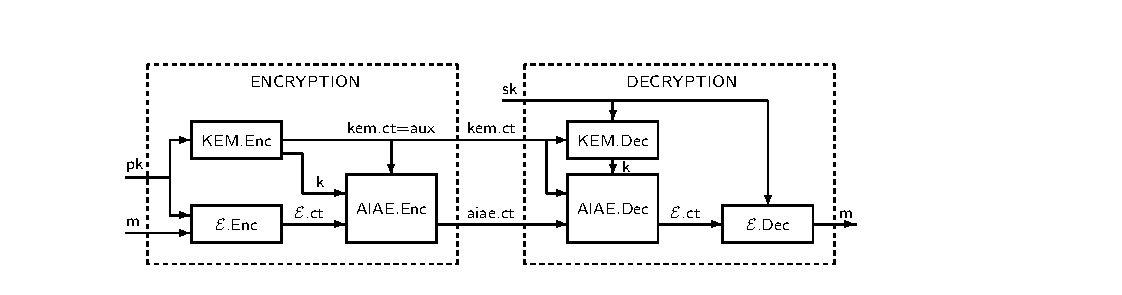
\includegraphics[height=4.5cm]{HanKEM.pdf}}
\caption{KDM-CCA安全公钥加密方案的通用设计方法
}\label{fig:KDMCCA-frame}
\end{figure}

在上述通用设计方法中, $\text{PKE}.\mathsf{Encrypt}$直接对消息$\mathsf{m}$进行加密. 特别地, 在$n$-KDM$[\F]$-CCA的实验中, $\text{PKE}.\mathsf{Encrypt}$直接加密依赖密钥消息$f(sk_1, \cdots, sk_n)$, 即$\mathsf{pke.ct} \leftarrow  \text{PKE}.\mathsf{Encrypt}(pk_j, f(sk_1, \cdots, sk_n))$, 其中$f \in \F$. 因此, 要求$\text{PKE}.\mathsf{Encrypt}$算法可以通过计算不可区分的变换, 使得$\mathsf{pke.ct}$中不含有私钥$(sk_1, \cdots, sk_n)$的特定信息, 从而私钥的一部分熵得到了保留.
这样的$\text{PKE}.\mathsf{Encrypt}$称为针对函数集合$\F$的熵过滤器(Entropy Filter).





\subsubsection{实例化方案}
使用前一节中的通用设计方法, 通过设计对应的组件KEM和组件PKE, 可以构造出支持仿射函数集合$\mathcal{F}_{\text{aff}}$和多项式函数集合$\mathcal{F}_{\text{poly}}^d$的KDM-CCA安全公钥加密方案。

\medskip\noindent\textbf{支持仿射函数集的KDM-CCA安全公钥加密方案.} 令$\text{AIAE}_{\text{DDH}} = (\text{AIAE}.\mathsf{Setup}, \text{AIAE}.\mathsf{Encrypt}, \text{AIAE}.\mathsf{Decrypt})$是前面构造的基于DDH假设的支持辅助输入认证加密方案, 其密钥空间为$(\mathbb{Z}_N)^4$、消息空间为$\mathcal{M}$. 根据图\ref{fig:KDMCCA-frame}中描述的KDM-CCA安全公钥加密方案的通用设计方法, 还需要构造另外两个组件:
\begin{itemize}
\item KEM: 针对具体的认证加密方案$\text{AIAE}_{\text{DDH}}$,需要设计一个密钥封装机制KEM,使得可以为$\text{AIAE}_{\text{DDH}}$方案封装一个密钥元组$(k_1, k_2, k_3, k_4) \in (\mathbb{Z}_N)^4$.

\item PKE: 针对仿射函数集合$\mathcal{F}{\text{aff}}$, 需要设计一个公钥加密方案PKE, 使得加密算法$\text{PKE}.\mathsf{Encrypt}$可以通过计算不可区分的变换, 转换成针对仿射函数的熵过滤器. 
\end{itemize}

公钥加密方案$\text{PKE} = (\mathsf{Setup}, \mathsf{KeyGen}, \mathsf{Encrypt}, \mathsf{Decrypt})$的具体描述见图\ref{fig:affinePKE}, 其中组件KEM和PKE的算法用灰色背景标注. 在初始化算法中, $pp_{\text{AIAE}}$中所包含的因子$p$和$q$没有提供给$pp_{\text{AIAE}}'$, 因为$p$和$q$不会在方案$\text{AIAE}_{\text{DDH}}$的加解密算法中使用.



{\renewcommand{\baselinestretch}{1.2} \normalsize
\begin{figure}[!h]
\centering
{\begin{tabular}{|l|l|}
\hline
~\makecell[l]{
\underline{$pp \leftarrow \textsf{Setup}(1^\kappa)$:}  \\
{$pp_{\text{AIAE}} \leftarrow \text{AIAE}.\mathsf{Setup}(1^\kappa)$, 其中} \\
{~~~~$pp_{\text{AIAE}} = (N,  p, q, \bar{N}, \bar{g}_1, \bar{g}_2, pp_{\text{AT}}, {\mathsf{TCR}})$,} \\
{~~~~$N = p q$, $\bar{N} = 2 N + 1$, $\bar{g}_{1}, \bar{g}_{2} \in \mathbb{QR}_{\bar{N}}$.} \\
{$pp_{\text{AIAE}}' := (N, \bar{N}, \bar{g}_1, \bar{g}_2, pp_{\text{AE}}, {\mathsf{TCR}})$.} \\
$g_1, g_2, g_3, g_4, g_5 \leftarrow \mathbb{SCR}_{N^s}$. \\
{Return~ $pp := (pp_{\text{AIAE}}', g_1, g_2, g_3, g_4, g_5 )$.} \\
\vspace{-5pt} \\
\underline{$\langle {\mathsf{aux}}, \mathsf{aiae.ct} \rangle \leftarrow \mathsf{Encrypt}(\mathsf{pk}, m)$:} ~$m \in \big[ N^{s-1} \big]$ \\
// $\big(\mathsf{k}, \mathsf{aux} \big) \leftarrow \text{KEM}.\mathsf{Encrypt}(\mathsf{pk})$: \\
\grabox{\makecell[l]{
$\mathsf{k} = (k_1, k_2, k_3, k_4) \sample (\mathbb{Z}_{N})^4$. \\
$r \leftarrow \big[ \big\lfloor \frac{N}{4} \big\rfloor \big]$. \\
$(u_1, u_2, u_3, u_4, u_5) := (g_1^{r}, g_2^{r}, g_3^{r}, g_4^{r}, g_5^{r})$ \\
~~~~$\bmod N^2$. \\
$(e_1, e_2, e_3, e_4) := (h_1^{r} T^{k_1}, h_2^{r} T^{k_2}, h_3^{r} T^{k_3},$ \\
~~~~$h_4^{r} T^{k_4}) \bmod N^2$. \\
$\mathsf{aux} := (u_1, \cdots, u_5, e_1, \cdots, e_4)$. \\ }~~~} \\
// $\mathsf{pke.ct} \leftarrow \text{PKE}.\mathsf{Enc}(\mathsf{pk}, m)$: \\
\grabox{\makecell[l]{
$\tilde{r}_1, \tilde{r}_2, \tilde{r}_3, \tilde{r}_4 \sample \big[ \big\lfloor \frac{N}{4} \big\rfloor \big]$. \\
$(\tilde{u}_1, \tilde{u}_2, \tilde{u}_3, \tilde{u}_4, \tilde{u}_5, \tilde{u}_6, \tilde{u}_7, \tilde{u}_8) := (g_1^{\tilde{r}_1}, g_2^{\tilde{r}_1},$ \\
~~~~$g_2^{\tilde{r}_2}, g_3^{\tilde{r}_2}, g_3^{\tilde{r}_3}, g_4^{\tilde{r}_3}, g_4^{\tilde{r}_4}, g_5^{\tilde{r}_4}) \text{~mod~} N^s$. \\
$\tilde{e} := h_1^{\tilde{r}_1} h_2^{\tilde{r}_2} h_3^{\tilde{r}_3} h_4^{\tilde{r}_4} T^m \bmod N^s$. \\
$t := g_1^m \bmod N  \in \mathbb{Z}_N$. \\
$\mathsf{pke.ct} := (\tilde{u}_1, \cdots, \tilde{u}_8, \tilde{e}, t)$. \\ }~} \\
$\mathsf{aiae.ct} \leftarrow \text{AIAE}.\mathsf{Encrypt}\big(\mathsf{k},  \mathsf{pke.ct}, \mathsf{aux} \big)$. \\
Return~ $\langle \mathsf{aux}, \mathsf{aiae.ct} \rangle$.  \\
}~     &
~\makecell[l]{
\underline{$(\mathsf{pk}, \mathsf{sk}) \leftarrow \mathsf{KeyGen}(pp)$:}  \\
$x_1, y_1, x_2, y_2, x_3, y_3, x_4, y_4 \sample \big[ \big\lfloor \frac{N^2}{4} \big\rfloor \big]$. \\
$(h_{1}, h_2, h_3, h_4) := (g_1^{- x_1} {g}_2^{- y_1}, g_2^{- x_2} {g}_3^{- y_2},$ \\
~~~~$g_3^{- x_3} {g}_4^{- y_3}, g_4^{- x_4} {g}_5^{- y_4}) \bmod N^s$. \\
$\mathsf{pk} := (h_{1}, h_{2}, h_3, h_4)$. \\
$\mathsf{sk} := ( x_1, y_1, x_2, y_2, x_3, y_3, x_4, y_4 )$.  \\
Return~ $(\mathsf{pk}, \mathsf{sk})$. \\
\vspace{-5pt} \\
\underline{$m / \bot \leftarrow \mathsf{Decrypt}\big(\mathsf{sk}, \langle {\mathsf{aux}}, \mathsf{aiae.ct} \rangle\big)$:} \\
// $\mathsf{k} / \bot \leftarrow \text{KEM}.\mathsf{Decrypt}(\mathsf{sk}, {\mathsf{aux}})$: \\
\grabox{\makecell[l]{
Parse~ $\textsf{aux} = (u_1, \cdots, u_5, e_1, \cdots, e_4)$. \\
If $e_1 u_1^{x_1} {u}_2^{y_1}, e_2 u_2^{x_2} {u}_3^{y_2}, e_3 u_3^{x_3} {u}_4^{y_3},$ \\
~~~$e_4 u_4^{x_4} {u}_5^{y_4} \in \mathbb{RU}_{N^2}$ \\
~~~~~$(k_1, k_2, k_3, k_4) := \big(\text{dlog}_T (e_1 u_1^{x_1} {u}_2^{y_1}),$ \\
~~~~~~$\text{dlog}_T (e_2 u_2^{x_2} {u}_3^{y_2}), \text{dlog}_T (e_3 u_3^{x_3} {u}_4^{y_3}),$ \\
~~~~~~$\text{dlog}_T (e_4 u_4^{x_4} {u}_5^{y_4})\big) \bmod N$. \\
~~~~~$\mathsf{k} := (k_1, k_2, k_3, k_4)$.  \\
Else, Return~ $\bot$. \\}}\\
$\mathsf{pke.ct} / \bot \leftarrow \text{AIAE}.\mathsf{Decrypt}\big( \mathsf{k}, \mathsf{aiae.ct}, \textsf{aux} \big)$.  \\
// $m / \bot \leftarrow \text{PKE}.\mathsf{Dec}(\textsf{sk}, \textsf{pke.ct})$: \\
\grabox{\makecell[l]{
Parse~ $\textsf{pke.ct} = (\tilde{u}_1, \cdots, \tilde{u}_8, \tilde{e}, t)$. \\
If $\tilde{e} \tilde{u}_1^{x_1} \tilde{u}_2^{y_1} \tilde{u}_3^{x_2} \tilde{u}_4^{y_2} \tilde{u}_5^{x_3} \tilde{u}_6^{y_3} \tilde{u}_7^{x_4} \tilde{u}_8^{y_4}  \in \mathbb{RU}_{N^s}$ \\
~~~~~$m := \text{dlog}_T (\tilde{e} \tilde{u}_1^{x_1} \tilde{u}_2^{y_1} \tilde{u}_3^{x_2} \tilde{u}_4^{y_2} \tilde{u}_5^{x_3} \tilde{u}_6^{y_3}$ \\
~~~~~~~$\tilde{u}_7^{x_4} \tilde{u}_8^{y_4})  \bmod N^{s-1}$. \\
~~~~~IF $t = g_1^m \text{~mod~} N$, ~Return~ $m$. \\
Else, Return~ $\bot$. \\}
} \\
}~      
\\
\hline
\end{tabular}}
\caption{支持仿射函数集合的KDM-CCA安全公钥加密方案PKE}\label{fig:affinePKE}
\end{figure}}


上述方案的安全性由以下定理保证.
\begin{theorem} \label{thm:PKE-KDM}
如果(i) $\text{AIAE}_{\text{DDH}}$是弱$\F_{\text{raff}}$-RKA安全的; (ii) $\mathsf{GenN}$算法的DCR假设成立; (iii) $\mathsf{GenN}$算法的DL假设成立. 则图\ref{fig:affinePKE}中构造的PKE方案是$n$-KDM$[\mathcal{F}{\text{aff}}]$-CCA安全的, 其中$n \in \mathbb{N}$表示用户数量、$\mathcal{F}{\text{aff}}$是仿射函数集合.
\end{theorem}

下面简要描述证明的思路, 详细分析请参考文献\cite{HLL-ASIACRYPT-2016}中定理2的证明.
\begin{enumerate}
    \item  对于$n$个用户的私钥$\mathsf{sk}_i =(x_{i,j}, y_{i,j})_{j = 1}^4$,$i \in [n]$,
         \begin{itemize}
         \item  每个私钥$\mathsf{sk}_i$(从信息论意义上)可以分为两个部分, 即
        模$N$的部分$(x_{i,j}, y_{i,j})_{j = 1}^4 \bmod N$和模$\phi(N)/4$的部分$(x_{i,j}, y_{i,j})_{j = 1}^4 \bmod \phi(N)/4$;
         \item  每个私钥$\mathsf{sk}_i$可以通过在一个固定的基私钥$(x_{j}, y_{j})_{j = 1}^4$上加随机偏移量$(\overline{x}_{i,j},$ $\overline{y}_{i,j})_{j = 1}^4$来生成, 即$\mathsf{sk}_i = (x_{i,j}, y_{i,j})_{j=1}^4 := (x_{j}, y_{j})_{j=1}^4 + (\overline{x}_{i,j}, \overline{y}_{i,j})_{j=1}^4$.
         \end{itemize}
    \item   每个用户的公钥$\mathsf{pk}_i =  (h_{i,1}, \cdots, h_{i,4})$只会泄露对应私钥$\mathsf{sk}_i$模$\phi(N)/4$部分的信息.

    \item 对于敌手的\textsc{Encrypt}查询$(i_\lambda, f_\lambda)$, 挑战密文可能通过$\mathsf{pek.ct}$部分泄露私钥$\mathsf{sk}_i$ ($i \in [\ell]$)的信息. 通过计算不可区分的变换, 能够保证\textsc{Encrypt}查询泄露的$\mathsf{sk}_i$的信息是有限的.
         \begin{itemize}
         \item 根据IV$_d$假设, 可以改变\textsc{Encrypt}查询中$\mathsf{pke.ct}$的生成方式, 使得$\mathsf{pke.ct}$不泄露任何关于$(x_{j}, y_{j})_{j = 1}^4 \bmod N$的信息, 即不泄露基私钥模$N$部分的信息.
         \item 根据IV$_d$假设, 可以改变\textsc{Encrypt}查询中$\mathsf{kem.ct}$($= \mathsf{aux}$)的生成方式, 使得其封装一个与$\text{AIAE}.\mathsf{Encrypt}$中使用的密钥不同的密钥.
           假设$\text{AIAE}.\mathsf{Encrypt}$使用的密钥是$\mathsf{k}_\lambda = (r_{\lambda}{k}^*_j+s_{\lambda,j})_{j = 1}^4$, 那么$\textsf{kem.ct}$($= \textsf{aux}$)中所封装的密钥则是$\big(r_\lambda \cdot (k^*_j - \alpha_j x_j - \alpha_{j+1} y_j) - r_\lambda \cdot (\alpha_j \bar{x}_{i_\lambda,j} + \alpha_{j+1} \bar{y}_{i_\lambda,j}) + s_{\lambda,j}\big)_{j = 1}^4 \bmod N$. 因此, $(k^*_1, \cdots, k^*_4)$现在被$(x_{j}, y_{j})_{j = 1}^4 \bmod N$保护了起来.
         \end{itemize}
         \item \textsf{Decrypt}查询也可能会泄露$(x_{j}, y_{j})_{j = 1}^4 \bmod N$的信息.
 通过计算不可区分的变换, 保证\textsf{Decrypt}查询可以不使用 $(x_{j}, y_{j})_{j = 1}^4 \bmod N$进行解密.   注意到敌手提交的密文只要满足$\forall {j\in [5]}, u_{j} \in \mathbb{SCR}_{N^2}$和$\forall {j\in [8]},  \tilde{u}_{j} \in \mathbb{SCR}_{N^s}$, 则\textsf{Decrypt}可以只用$\phi(N)$和私钥$\mathsf{sk}_i$模$\phi(N)/4$部分的信息来完成解密过程.
         \begin{itemize}
         \item 如果敌手提交的密文使得$\exists j \in [5], u_{j} \notin \mathbb{SCR}_{N^2}$, 则根据$\text{AIAE}_{\text{DDH}}$的弱INT-$\F_{\text{raff}}$-RKA安全性, 可以证明$\text{AIAE}.\mathsf{Decrypt}$解密失败并输出$\bot$.        
         \item 如果敌手提交的密文使得$\exists j \in [8], \tilde{u}_{j} \notin \mathbb{SCR}_{N^s}$, 可以证明$t\neq g_1^m \bmod N$, 从而$\text{PKE}.\mathsf{Decrypt}$解密失败并输出$\bot$.
         \end{itemize}
         \item 因此, $(x_{j}, y_{j})_{j = 1}^4 \bmod N$和$(k^*_1, \cdots, k^*_4)$对于敌手而言都是均匀分布的. 此外, $\text{AIAE}.\mathsf{Encrypt}$总是使用$\mathsf{k}^* = (k^*_1, \cdots, k^*_4)$的受限仿射函数值作为密钥进行加密, 故再根据$\text{AIAE}_{\text{DDH}}$的IND-$\F_{\text{raff}}$-RKA安全性, PKE的$n$-KDM$[\F_{\text{aff}}]$-CCA安全性得证.
\end{enumerate}

\begin{note}
IV$_d$假设可以看作是扩展的Paillier密文在加密$0$向量和敌手指定的消息向量是不可区分的. 扩展的Paillier加密方案的密文形式是$g^r(1+N)^m \bmod N^{s+1}$, 其中$s \geq 2$, $g$是$\mathbb{Z}_{N^{s+1}}^*$上的$N^s$次剩余元素, 具体可参考文献~\cite{BG2010}.
\end{note}

\medskip\noindent\textbf{支持多项式函数集的KDM-CCA安全公钥加密方案.} 针对有界多项式函数集合$\F_{\text{poly}}^{d}$设计KDM-CCA安全的公钥加密方案, 其中$d$表示多项式函数集合里多项式函数的最大次数, $d$可以是安全参数$\kappa$的任意多项式, 仍然遵循图~\ref{fig:KDMCCA-frame}中描述的通用设计方法, 即通过构造三个组件KEM、PKE和AIAE. 该方案与前面介绍的支持仿射函数集合的KDM-CCA安全公钥加密方案(参见图\ref{fig:affinePKE})共享相同的组件KEM和组件$\text{AIAE}_{\text{DDH}}$. 为了使KDM-CCA安全性支持所有有界次数的多项式函数, 需要重新设计组件PKE, 使其加密算法$\text{PKE}.\mathsf{Encrypt}$可以通过计算不可区分的变换, 转换成针对多项式函数的熵过滤器. 设计此类PKE组件的基本技术是多项式降元技术. Han等人提出的降元技术可以将KDM询问的多项式函数的可能项式复杂度从$\binom{8n+d}{8n} = \Theta(d^{8n})$降至$\binom{8+d}{8} = \Theta(d^{8})$. 由于该方案的描述较复杂, 在此不再赘述. 详细内容可参考文献~\cite{HLL-ASIACRYPT-2016}第6节.



\subsection{QLH13方案}
2001年, Camenisch和Lysyanskaya~\cite{CL-EUROCRYPT-2001}提出一个实用的匿名证书系统. 在该系统中, 为了阻止用户将自己的密钥分享给他人使用, 作者提出通过循环加密私钥来实现``all-or-nothing sharing''的性质: 一个用户若允许别人使用他的私钥, 则别人可以得到他的所有证书(具体指方案的私钥). 通常,$n$个用户的循环加密方案包含以下$n$个密文: $\{\mathsf{Encrypt}(pk_i,sk_{i+1\bmod n})\}_{i\in[n]}$. 显而易见, 若知道一个私钥, 通过该组密文可以得到所有用户的私钥.

2013年, Qin等人~\cite{Qin-ACISP-2013}指出, 实现``all-or-nothing sharing''性质也可通过如下形式的循环加密实现, 从而设计了一个具有KDM-CCA安全性的$\mathsf{CS}$方案. 除了需要对加密的消息重新编码外, 方案的结构与原始CS方案完全相同, 具有更好的应用价值.
\[
\mathsf{Encrypt}(pk_1, sk_1 - sk_2), \mathsf{Encrypt}(pk_2, sk_2 - sk_3),\ldots,\mathsf{Encrypt}(pk_n, sk_n-sk_1).
\]

\subsubsection{KDM函数族定义}\label{sec:ch5-Function}
令$L := \mathsf{poly}(\kappa)$和$M := \mathsf{poly}(\kappa)$为两个正整数, $q$为一个素数. 令$\mathcal{X}$为$\mathbb{Z}_q$的一个有限子集. 环$\mathbb{Z}_q$上的函数族$\mathcal{F}_{q, n}^{L, M}: \mathcal{X}^n \rightarrow \mathbb{Z}_q$定义如下: 对于任意$f \in \mathcal{F}_{q,n}^{L,M}$, 函数$f$的表达式如下: 
\begin{displaymath}
f(x_1, \ldots, x_n) = \sum_{t=1}^{L} \prod_{i, j \in [n]}\alpha_{i, j, t}(x_i - x_j)^{a_{i, j, t}}\pmod q,
\end{displaymath}
其中$\alpha_{i, j, t} \in \mathbb{Z}_q$, $\sum_{i, j \in [n]}a_{i, j, t} \leq M$. 实际上, $f$可以看做是一个以$n^2$个$\{x_i - x_j\}_{i, j\in [n]}$为变量的多变量函数. 令$\mathcal{S}(n^2)$表示环$\mathbb{Z}_q$上所有具有$n^2$个变量的多项式, 则
\[
\mathcal{F}_{q, n}^{L, M} = \{g: (x_i - x_j)_{i, j \in [n]} \rightarrow \mathbb{Z}_q ~|~  g \in \mathcal{S}(n^2), x_i \in \mathcal{X}, i\in [n]\}.
\]

显然, 集合$\mathcal{F}_{q, n}^{L, M}$包含$(x_1 - x_2), (x_2 - x_3), \ldots, (x_{n-1} - x_n),(x_n - x_1)$这些特殊的函数. 由此可得
\begin{displaymath}
   \left( \begin{array}{c}
      x_1 - x_2      \\
      x_2 - x_3      \\
      \vdots         \\
      x_{n-1} - x_n  \\
      x_n-x_1
    \end{array}\right)=\underbrace{\left(\begin{array}{cccccc}
                  1      & -1     & 0      &\ldots  & 0      & 0      \\
                  0      & 1      & -1     &\ldots  & 0      & 0      \\
                  \vdots & \vdots & \vdots & \ldots & \vdots & \vdots \\
                  0      & 0      & 0      &\ldots  & 1      & -1     \\
                 -1      & 0      & 0      &\ldots  & 0      & 1
                \end{array}\right)}_{A}\cdot
                \left(\begin{array}{c}
                  x_1     \\
                  x_2     \\
                  \vdots  \\
                  x_n
                \end{array}\right).
    \end{displaymath}
其中矩阵$A_{n \times n}$的秩为$n$.

对于任意向量$\vec{b} = (b_1, b_2, \ldots, b_n) \in \mathbb{Z}_q^n$和$\beta \in \mathbb{Z}_q$, 函数
\[
f(x_1, x_2, \ldots, x_n) = (b_1, b_2, \ldots, b_n) \cdot A \cdot
                \left(\begin{array}{c}
                  x_1      \\
                  x_2      \\
                  \vdots   \\
                  x_n
                \end{array}\right) + \beta
\] 
构成一个仿射函数且属于函数集合$\mathcal{F}_{q, n}^{L, M}$.

令$\mathcal{I} = \{\vec{b} \cdot A \cdot  (x_1, x_2, \ldots, x_n)^T + \beta ~|~\vec{b} \in \mathbb{Z}_q^n, \beta \in \mathbb{Z}_q\}$, $\Gamma$为所有从$\mathcal{X}^n$到$\mathbb{Z}_q$的仿射函数集合. 则$\mathcal{I} = \mathcal{F}_{q, n}^{L,M} \cap  \Gamma$. 因此,新定义的函数集合不仅包含了部分仿射函数, 而且当多项式的次数大于1时, 该函数集合还包含了许多不属于仿射函数的一般函数, 见图~\ref{fig:ch5-1}。
\begin{figure}[h]
\centering
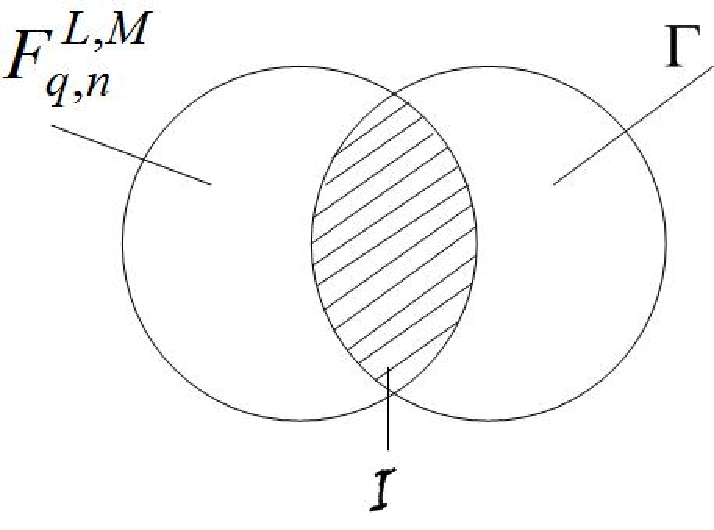
\includegraphics[width=50mm]{figure/KDM-Fun.pdf}
\caption{函数族之间的关系} \label{fig:ch5-1}
\end{figure}

当考虑依赖密钥消息加密安全性时, 集合$\mathcal{X}$替换为私钥空间$\mathcal{K}$, 而函数族定义为
 $\mathcal{F}_{q, n}^{L, M} = \{g: (sk_i - sk_j)_{i, j \in [n]} \rightarrow \mathbb{Z}_q ~|~  g \in \mathcal{S}(n^2), sk_i\in \mathcal{K}, i\in [n]\}$. 当计算某一元素的函数值时, 默认假设$\mathcal{K} \subseteq \mathbb{Z}_q$.

如果$\mathcal{K} \nsubseteq \mathbb{Z}_q$, 我们假设存在一个有效的单射函数将$\mathcal{K}$映射到$\mathbb{Z}_q$的一个向量空间上. 所有私钥$sk_i$被替换为$\mathbb{Z}_q$上的某个向量.

\subsubsection{KDM-CCA安全的Cramer-Shoup方案}\label{sec:ch5-KDMCS}
Cramer-Shoup方案~\cite{CramerS03}的消息空间是一个阶为素数$q$的有限循环群$\mathbb{G}$, 而私钥空间为$\mathbb{Z}_q^6$. 为了把私钥作为消息进行加密, 必须将方案的密钥$sk = (x_1, x_2, x_3, x_4, x_5, x_6) \in \mathbb{Z}_q^6$编码为群$\mathbb{G}$上的六个元素. 假设存在一个有效的编码算法$\mathsf{Encode}: \mathbb{Z}_q \rightarrow \mathbb{G}$和解码算法$\mathsf{Decode}:  \mathbb{G} \rightarrow \mathbb{Z}_q$并且对于所有$x\in \mathbb{Z}_q$满足$\mathsf{Decode}(\mathsf{Encode}(x)) = x$. 下面, 给出这种编码算法的一种具体构造.


基于上述消息编码的Tailored Cramer-Shoup加密方案$\text{TCS} = (\mathsf{Setup}, \mathsf{KeyGen}, \mathsf{Encrypt}, \mathsf{Decrypt})$如构造~\ref{construction:ch5-KDMCS}所示.

\begin{construction}[Tailored Cramer-Shoup加密方案]\label{construction:ch5-KDMCS}
\begin{itemize}
\item $\mathsf{Setup}(1^\kappa)$: 选择一个阶为素数$q$的有限循环群$\mathbb{G}$, 两个随机生成元$g,\hat{g} \sample \mathbb{G}$及一个目标抗碰撞哈希函数$\mathsf{H}: \mathbb{G}^3 \rightarrow \mathbb{Z}_q$. 返回系统参数$pp = (q,\mathbb{G}, g, \hat{g}, \mathsf{H})$.

\item $\mathsf{KeyGen}(pp)$: 随机选择$(x_1,\ldots, x_6) \sample \mathbb{Z}_q^6$并计算
\begin{align*}
h_1 & = g^{x_1} \hat{g}^{x_2} & \qquad h_2 & = g^{x_3} \hat{g}^{x_4} & \qquad h_3 & = g^{x_5}\hat{g}^{x_6}.
\end{align*}
返回公钥$pk = (h_i)_{i\in[3]}$和私钥$sk = (x_i)_{i \in [6]}$.

\item $\mathsf{Encrypt}(pk, m)$: 将公钥$pk$展开为$(h_1, h_2, h_3)$. 对于消息$m \in \mathbb{Z}_q$, 随机选择$r \sample \mathbb{Z}_q$并计算
\begin{displaymath}
u = g^r, \qquad \hat{u} = \hat{g}^r, \qquad c = h_1^r \cdot \mathsf{Encode}(m), \qquad v = (h_2^th_3)^r
\end{displaymath}
其中$t = \mathsf{H}(u, \hat{u}, c)$. 返回密文$C = (u, \hat{u}, c, v)$.

\item $\mathsf{Decrypt}(sk, C)$: 首先, 将私钥$sk$展开为$(x_i)_{i = 1}^6$, 密文$C$展开为$(u,\hat{u}, c, v)$. 计算$t = \mathsf{H}(u, \hat{u}, c)$并验证$u^{x_3t + x_5} \cdot \hat{u}^{x_4t + x_6} \overset{?}{=} v$是否成立. 若不成立, 返回$\bot$; 否则返回$\mathsf{Decode}(c/u^{x_1}\hat{u}^{x_2})$.
\end{itemize}
\end{construction}

在Tailored Cramer-Shoup加密方案中, 消息编码算法和解码算法的具体构造如下:
\begin{itemize}[noitemsep,topsep=0pt]
\item 系统参数$\mathsf{Setup}(1^\kappa)$: 选择一个安全素数$p=2q+1$, 即$p$和$q$都为素数. 令$\mathbb{G} = \mathbb{QR}_p$表示$\mathbb{Z}_p^*$的二次剩余群. 选择两个随机生成元$g,\hat{g} \in \mathbb{QR}_p$. 则系统参数为$pp = (p, q, \mathbb{QR}_p, g, \hat{g})$.

\item 编码算法$\mathsf{Encode}(x)$: 令$\left(\frac{x}{p}\right)$表示Legendre符号. 则编码算法$\mathsf{Encode}: \mathbb{Z}_q \rightarrow \mathbb{QR}_p$定义为:
\begin{displaymath}
\mathsf{Encode}(x) := \left\{\begin{array}{ll}
x,   & \textrm{ if } \left(\frac{x}{p}\right) = 1  \\
p-x, & \textrm{ if } \left(\frac{x}{p}\right) = -1
\end{array}
\right.
\end{displaymath}

\item 解码算法$\mathsf{Decode}(y)$: 解码算法$\mathsf{Decode}: \mathbb{QR}_p \rightarrow \mathbb{Z}_q$定义为:
\[
\mathsf{Decode}(y) := \left\{\begin{array}{ll}
  y, & \textrm{ if } 1 \leq  y \leq q \\
p-y, & \textrm{ if } q < y \leq p-1
\end{array}
\right.
\]
\end{itemize}

在上述编码/解码算法中, 对于每个$x \in \mathbb{Z}_q$, 如果$\left(\frac{x}{p}\right) = 1$, 则 $x \in \mathbb{QR}_p$; 如果$\left(\frac{x}{p}\right) = -1$, 则$\left(\frac{p - x}{p}\right) = 1$. 因此, $p - x \in \mathbb{QR}_p$. 对于不同的$x_1, x_2 \in \mathbb{Z}_q$, 可知$\mathsf{Encode}(x_1) \neq \mathsf{Encode}(x_2)$. 故, $\mathsf{Encode}$是一个双射. 类似地, 可以验证$\mathsf{Decode}$是相应的逆映射.

\begin{trivlist}
\item \textbf{正确性.} 对于消息$m$的密文$C = (u, \hat{u}, c, v)$, 我们有
\begin{displaymath}
\left\{\begin{array}{l}
u^{x_3t + x_5} \cdot \hat{u}^{x_4t + x_6} = (g^{x_3}\hat{g}^{x_4})^{tr} \cdot (g^{x_5}\hat{g}^{x_6})^r = (h_2^th_3)^r = v\\\\
\mathsf{Decode}\left(\dfrac{c}{u^{x_1}\hat{u}^{x_2}}\right) = \mathsf{Decode}\left(\dfrac{h_1^r \cdot \mathsf{Encode}(m)}{h_1^r}\right) = \mathsf{Decode}(\mathsf{Encode}(m))=m
\end{array}\right..
\end{displaymath}
由此说明Tailored Cramer-Shoup加密方案是正确的.
\end{trivlist}

\begin{trivlist}
\item \textbf{KDM-CCA安全性.} 方案的安全性由下面的定理保证:
\begin{theorem}\label{thm:ch5-TCS}
对于任意正整数$n\geq 2$, $L$和$M$, 实例化的Cramer-Shoup方案相对于函数集$\mathcal{F}_{q,n}^{L,M}$是KDM-CCA安全的. 具体可得:
\begin{displaymath}
\mathsf{Adv}_{\text{TCS}, \mathcal{A}}^{\textup{kdm-cca}}(\kappa) \leq 2nQ_e \cdot \left(\mathsf{Adv}_{\mathbb{QR}_p, \mathcal{D}}^{\textup{ddh}}(\kappa) + \mathsf{Adv}_{\mathsf{H},\mathcal{B}}^{\textup{tcr}}(\kappa) + \frac{(Q_d+4)}{q}\right)
\end{displaymath}
这里我们假设$\mathcal{A}$最多询问$Q_e$次加密服务和$Q_d$次解密服务.
\end{theorem}
\end{trivlist}

\begin{proof}
我们仅给出定理的证明思路, 具体证明可参考文献~\cite{Qin-ACISP-2013}.

由于Tailored CS加密方案与原始的CS加密方案仅在消息的形式上不同, 因此该方案仍然是IND-CCA安全的. 要证明它的KDM-CCA安全性, 我们只需要给出模拟私钥函数$f(sk)$加密谕言机的方法. 假设$n$个用户的私钥分别为$sk_i = (x_{i,1}, x_{i,2}, x_{i,3}, x_{i,4}, x_{i,5}, x_{i,6})$ ($i = 1, 2,\ldots, n.$). 则方案将私钥变换为消息的KDM函数族$\mathcal{F}_{q, n}^{L, M}$的具体形式如下:
\begin{eqnarray*}
f(sk_1, \ldots, sk_n) &=& f((x_{i,1}, x_{i,2}, x_{i,3}, x_{i,4}, x_{i,5}, x_{i,6})_{i = 1}^{n})\\
                      &=& \sum_{t=1}^{L} \prod_{i, j \in [n], s \in [6]} \alpha_{i,j,t}(x_{i,s} - x_{j,s})^{a_{i,j,t}}\pmod q,
\end{eqnarray*}
其中$\alpha_{i,j,t} \in \mathbb{Z}_q$, $a_{i,j,t} \in \mathbb{N}$.

我们知道, 公钥和私钥的形式分别为$pk = (h_i)_{i=1}^3 = \left(g^{x_{2i-1}}\hat{g}^{x_{2i}}\right)_{i = 1}^3$和$sk = (x_i)_{i = 1}^6$, 其中$g, \hat{g}$是随机选取的生成元, $(x_i)_{i = 1}^6$是从$\mathbb{Z}_q$中独立选取的. 当使用公钥$pk$加密消息$m \in \mathbb{Z}_q$时, 先选取随机数$r \in \mathbb{Z}_q$, 再计算密文$C = (u, \hat{u}, c, v) = (g^r, \hat{g}^r, h_1^r \cdot \mathsf{Encode}(m), h_2^{rt}h_3^r)$, 其中$t = \mathsf{H}(u, \hat{u}, c)$. 而在证明过程中, 模拟者可以通过一个公钥/私钥对$(pk^*, sk^*)$来生成其他$n$个用户的公钥. 首先, 模拟者随机选取差值$\widehat{sk_i} \in \mathbb{Z}_q^6$, 并利用这些差值和公钥$pk^*$构造新的公钥$pk_i$且相应的私钥为$sk_i = sk^* + \widehat{sk_i}$. 模拟者虽然不知道$pk_i$对应的真正私钥, 但是对于任意两个用户的私钥之差是可以计算出来的. 因此, 模拟者可以完美地计算任意KDM函数$f \in \mathcal{F}_{q, n}^{L, M}$的值$f(sk_1, \ldots, sk_n)$, 从而完美模拟KDM加密谕言机. 对于敌手的解密询问, 假设密文$C = (u, \hat{u}, c, v)$是使用公钥$pk_i$加密某一消息$m$得到的. 那么, 模拟者可以构造一个使用公钥$pk^*$加密另一消息$m^*$的密文$C^* = (u, \hat{u}, c, v^*)$, 并且利用$m^*$恢复真正的消息$m$. 由此可知, 模拟者可以利用自己的挑战者提供的解密服务(私钥$sk^*$对应的解密谕言机)来获得消息$m^*$, 从而恢复出原始消息. 这说明Tailored CS加密方案的KDM-CCA安全性可以归约到自身的IND-CCA安全性上. 
\end{proof}


